\subsection{Example: Error in evaluating the trajectory}

In practical engineering, we often need to evaluate the difference between the estimated trajectory of an algorithm and the real trajectory to evaluate the accuracy of the algorithm. The true trajectory is often obtained by some higher precision systems, and the estimated estimate is calculated by the algorithm to be evaluated. In the previous chapter we demonstrated how to display a track stored in a file. In this section we will consider how to calculate the error of two tracks. Consider an estimated trajectory $\bm{T}_{\mathrm{esti}, i}$ and the real trajectory $\bm{T}_{\mathrm{gt},i}$, where $i=1,\cdots , N$, then we can define some error indicators to describe the difference between them.

There are many kinds of error indicators. The common one is \textbf{Absolute Trajectory Error} (ATE), which is like:

\begin{equation}
\mathrm{ATE}_{\mathrm{all}} = \sqrt{ \frac{1}{N} \sum_{i=1}^N \| \log( \bm{T}_{\mathrm{gt },i}^{-1} \bm{T}_{\mathrm{esti},i} )^{\vee} \|_2^2},
\end{equation}

This is actually the \textbf{root mean square error} (Root-Mean-Squared Error) (RMSE) for each pose Lie algebra. This error can characterize the rotation and translation errors of the two tracks. At the same time, some literatures only consider the translation error \cite{Sturm2012}, so you can define \textbf{Average Translational Error}:

\begin{equation}
\mathrm{ATE}_{\mathrm{trans}} = \sqrt{ \frac{1}{N} \sum_{i=1}^N \| \mathrm{trans}( \bm{T}_{\ Mathrm{gt},i}^{-1} \bm{T}_{\mathrm{esti},i} ) \|_2^2},
\end{equation}

Where $\mathrm{trans}$ represents the translation of the internal variables of the parentheses. Because from the perspective of the entire trajectory, after the error occurs in the rotation, the subsequent trajectory will also have an error in the translation, so both indicators are applicable in practice.

In addition to this, relative errors can also be defined. For example, consider the movement from $i$ to the time of $i+\Delta t$, then the Relative Pose Error (RPE) can be defined as:

\begin{equation}
\mathrm{RPE}_{\mathrm{all}} = \sqrt{ \frac{1}{N-\Delta t} \sum_{i=1}^{N-\Delta t} \| \log \left ( \left(\bm{T}_{\mathrm{gt},i}^{-1} \bm{T}_{\mathrm{gt},i+\Delta t} )\right)^{-1 } \left(\bm{T}_{\mathrm{esti},i}^{-1} \bm{T}_{\mathrm{esti},i+\Delta t}\right)\right)^{ \vee} \|_2^2},
\end{equation}

Similarly, you can only take the translation part:

\begin{equation}
\mathrm{RPE}_{\mathrm{trans}} = \sqrt{ \frac{1}{N-\Delta t} \sum_{i=1}^{N-\Delta t} \| \mathrm{trans } \left( \left(\bm{T}_{\mathrm{gt},i}^{-1} \bm{T}_{\mathrm{gt},i+\Delta t} )\right)^ {-1} \left(\bm{T}_{\mathrm{esti},i}^{-1} \bm{T}_{\mathrm{esti},i+\Delta t}\right)\right ) \|_2^2}.
\end{equation}

This part of the calculation is easy to implement with the Sophus library. Below we demonstrate the calculation of the absolute trajectory error. In this example, we have two tracks, groundtruth.txt and estimated.txt. The following code will read the two tracks, calculate the error, and display it in the 3D window. For the sake of brevity, the code for the trajectory portion has been omitted, and we have done similar work in the previous lecture.
\begin{lstlisting}[language=c++,caption=slambook/ch4/example/trajectoryError.cpp(part)]
#include <iostream>
#include <fstream>
#include <unistd.h>
#include <pangolin/pangolin.h>
#include <sophus/se3.hpp>

Using namespace Sophus;
Using namespace std;

String groundtruth_file = "./example/groundtruth.txt";
String estimated_file = "./example/estimated.txt";

Typedef vector<Sophus::SE3d, Eigen::aligned_allocator<Sophus::SE3d>> TrajectoryType;

Void DrawTrajectory(const TrajectoryType >, const TrajectoryType &esti);

TrajectoryType ReadTrajectory(const string &path);

Int main(int argc, char **argv) {
TrajectoryType groundtruth = ReadTrajectory(groundtruth_file);
TrajectoryType estimated = ReadTrajectory(estimated_file);
Assert(!groundtruth.empty() && !estimated.empty());
Assert(groundtruth.size() == estimated.size());

// compute rmse
Double rmse = 0;
For (size_t i = 0; i < estimated.size(); i++) {
Sophus::SE3d p1 = estimated[i], p2 = groundtruth[i];
Double error = (p2.inverse() * p1).log().norm();
Rmse += error * error;
}
Rmse = rmse / double(estimated.size());
Rmse = sqrt(rmse);
Cout << "RMSE = " << rmse << endl;

DrawTrajectory(groundtruth, estimated);
Return 0;
}

TrajectoryType ReadTrajectory(const string &path) {
Ifstream fin(path);
TrajectoryType trajectory;
If (!fin) {
Cerr << "trajectory " << path << " not found." << endl;
Return trajectory;
}

While (!fin.eof()) {
Double time, tx, ty, tz, qx, qy, qz, qw;
Fin >> time >> tx >> ty >> tz >> qx >> qy >> qz >> qw;
Sophus::SE3d p1(Eigen::Quaterniond(qx, qy, qz, qw), Eigen::Vector3d(tx, ty, tz));
Trajectory.push_back(p1);
}
Return trajectory;
}
\end{lstlisting}

The result of this program output is 2.207, and the image is shown as \autoref{fig:trajectory-compare}. The reader also tries to remove the rotating part and only calculates the error of the translation part. For this example, we have actually helped the reader to do some pre-processing tasks, including time alignment of the trajectory and external parameter estimation. These contents have not been mentioned yet, and we will talk about it in future learning.

\begin{figure}[!ht]
	\centering
	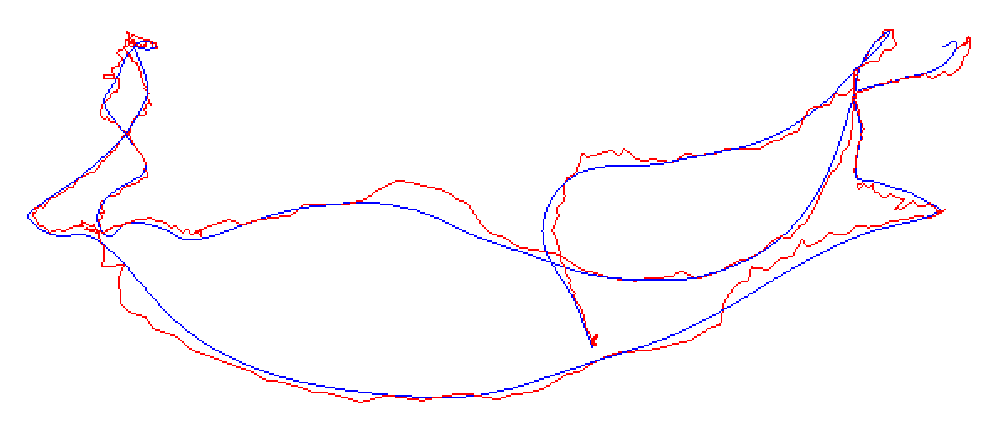
\includegraphics[width=1.0\textwidth]{chapter05/lieGroup/trajectory-compare.pdf}
	\caption{calculates the error between the estimated trajectory and the real trajectory. }
	\label{fig:trajectory-compare}
\end{figure}